\subsection{Analyse des performances}

Dans cette section nous allons mener une analyse des performances de chaque solution, en termes de quantité de trafic que les machines sont capables de traiter. En raison de l'utilisation massive des algorithmes de chiffrement et déchiffrement, c'est la capacité processeur des machines qui sera déterminante.

Nous avons utilisé un outil Open-Source afin de mener à bien cette évaluation des performances. Ce logiciel très simple nommé IPperf envoie simplement la quantité désirée de paquets d'un point à un autre.

\subsubsection{Configuration d'IPperf}

Le but de ce benchmark est de générer du trafic et de forcer son passage à travers le tunnel VPN. Pour pouvoir effectuer des mesures, IPperf doit être lancé sur une machine cliente d'un côté du tunnel, ainsi que sur une machine serveur de l'autre côté :

\begin{figure}[H]
	\begin{center}
		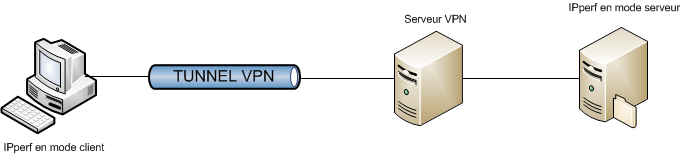
\includegraphics[width=0.75\textwidth]{partie_3/images/ipperf.png}\\
	\end{center}
	\caption{Protocole de test}
	\label{Protocole_de_test}
\end{figure}

Voici la configuration d'IPperf :
En mode serveur : \verb|iperf.exe -s -i1|. L'option \verb|-s| correspond au mode serveur et le \verb|-i1| correpond à la fréquence de prise de mesure (ici une seconde).

En mode client : \verb|iperf.exe -c 10.0.1.25 -i1 -t40 |. L'option \verb|-c| correspond au mode client et l'option \verb|-t40| indique la durée pendant laquelle on va générer du trafic.

\subsubsection{Confrontration des résultats}

Voici les caractéristiques de la plateforme ayant fait office de serveur :
\begin{figure}[H]
	\begin{center}
\begin{tabular}{l|c}
Caractéristiques & Machine \\
\hline
CPU & Intel Core 2 Duo T8100 2,10GHz \\
RAM & 3 Go \\
Carte réseau & Intel 82566MM Gigabit \\
\end{tabular}
	\end{center}
	\caption{Caractéristiques de la plateforme serveur}
	\label{Caractéristique_de_la_plateforme_serveur}
\end{figure}

Les machines clientes utilisées sont celles présentes en salle A214. La figure \ref{Résultat_des_benchmarks} présente les résultats que nous avons obtenus. La bande passante indiqué correspond à une moyenne sur quarante secondes :

\begin{figure}[H]
	\begin{center}
\begin{tabular}{l|c|c|c}
Solution & WINDOWS & LINUX & CISCO \\
\hline
Bande Passante & 18Mbps & 50Mbps & 31Mbps \\
Utilisation CPU & 100\% & 80\% & 100\% \\
\end{tabular}
	\end{center}
	\caption{Résultats des benchmarks}
	\label{Résultat_des_benchmarks}
\end{figure}

Le taux d'utilisation processeur n'est pas fournit par IPperf. Cette valeur a été obtenue directement en visualisant la charge de la machine. Dès lors que du trafic traverse le tunnel, les serveurs VPN se trouvent fortement sollicités, et il devient rapidement très difficile d'exécuter une autre tâche en parallèle. Comme prévu, le taux d'occupation processeur est le facteur limitant pour chaque solution, ce dernier étant responsable du traitement des packets transitant sur réseau.

En terme de bande passante, la solution OpenVPN se révèle être la plus performante. Cependant, nous avons remarqué des fluctuations durant les mesures, ce qui n'est pas le cas du routeur CISCO dont le débit est extrêment stable.
